\documentclass{article}
    \usepackage[utf8]{inputenc}
    \usepackage[T2A]{fontenc}
    \usepackage[english,russian]{babel}

    % Related to math
    \usepackage{amsmath,amssymb,amsfonts,amsthm}

    \usepackage{graphicx}
    \graphicspath{{media/}}

\begin{document}

\section{Моделирование маршрута инструмента для машин фигурной листовой резки с ЧПУ. Основные понятия и задачи}

\subsection{Технологии и техники листовой резки на машинах с ЧПУ}

В машиностроении, в производстве металлоконструкций
и в других отраслях промышленности существенная часть продукции
зготавливается из заготовок,
получаемых из листовых материалов на различном технологическом оборудовании.
К такому оборудованию относятся, в частности,
Используемые на предприятиях отечественные и зарубежные
системы автоматизированного проектирования (САПР),
предназначенные для разработки управляющих программ (УП)
для машин листовой резки с ЧПУ (т.н. Computer-Aided Manufacturing, CAM-системы)
обеспечивают автоматизацию процесса разработки УП,
однако не позволяют решить многие оптимизационные задачи.
При этом при моделировании маршрута инструмента пользователям
САПР часто приходится применять интерактивные методы проектирования УП,
поскольку алгоритмы генерации УП,
реализованные в автоматическом режиме проектирования,
во многих случаях не позволяет генерировать оптимальные управляющие программы,
а также обеспечить соблюдение некоторых технологических требований листовой резки.
В качестве критериев оптимизации имеются в виду время резки и
некоторые другие стоимостные характеристики процесса листовой резки.
Проблема разработки методов, алгоритмов и соответствующего программного обеспечения,
позволяющих в автоматическом режиме оптимизировать параметры
процесса резки заготовок из листовых материалов на машинах с числовым программным управлением,
включая алгоритмы маршрутизации движения инструмента,
которые бы обеспечивали минимизацию времени резки и стоимости процесса,
остается актуальнейшей задачей раскройно-заготовительного производства.

Рассмотрим понятие маршрута инструмента (маршрута резки)
применительно к некоторым технологиям фигурной листовой резки.
В настоящее время в промышленном производстве
единичного и мелкосерийного типа для раскроя листовых материалов
используются в основном следующие технологии:
лазерная, плазменная, газовая и гидроабразивная.
Целесообразность их применения определяется различными технологическими факторами,
например, свойствами раскраиваемого материала,
экономическими требованиями к процессу резки,
требованиями к качеству реза и пр.
Эти и некоторые другие технологии резки предполагают,
что для сохранения требуемой геометрии заготовки
траектория движения режущего инструмента не совпадает
с граничным контуром заготовки,
а задается некоторой эквидистантой этого контура,
поскольку часть материала вырезается («сгорает», «вымывается» и пр.)
в процессе резки.
Как правило, дистанция между эквидистантным контуром,
по которому осуществляется резка, и граничным контуром заготовки определяется величиной,
равной половине ширины реза.
Эта величина зависит от выбранной технологии резки,
толщины и марки материала, заданной скорости резки
и особенностей конкретного технологического оборудования,
используемого для резки.

Еще она особенность листовой резки –
необходимость предварительной врезки (пробивки)
материала перед процессом резки непосредственно
по эквидистантному контуру заготовки.
Пробивка материала сопровождается дополнительными
деформациями материала в точке врезки,
поэтому производится на расстоянии (дистанции)
от контура заготовки большем,
чем дистанция до эквидистантного контура за исключением случаев,
когда для точек врезки в листовом материале механическим способом
готовятся (например, просверливаются)
отверстия.
Врезка может также осуществляться
непосредственно на границе материала
(«врезка с края листа»).
В этом случае достигается уменьшение
деформаций материала и сокращается время врезки.

Один из способов резки заготовки (стандартная техника)
показан на Рис. \ref{standard-cutting}.

\begin{figure}
  \begin{center}
  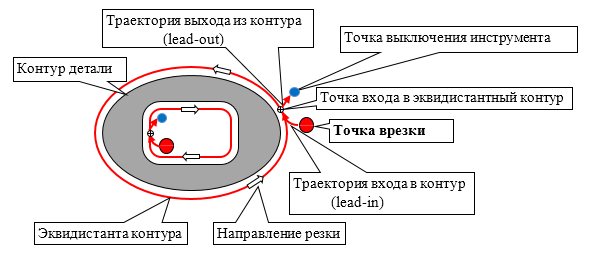
\includegraphics[width=0.9\textwidth]{cutting-path.png}
  \caption{Схема стандартной техники резки (резка по замкнутому контуру)}
  \label{standard-cutting}
  \end{center}
\end{figure}

\end{document}
